\documentclass{acm_proc_article-sp}
\usepackage{verbatim}
\usepackage{graphicx}
\begin{document}

\title{Learning PSRs with The Base System}

\numberofauthors{1}

\author{
\alignauthor
Lucas Langer\\
\email{lucas.langer@mail.mcgill.ca}
}

\date{12 August 2015}

\maketitle

\section{Problem and Motivation}

We consider the problem of learning models of time series data in partially observable environments. Typical applications arise in robotics and reinforcement learning, where hidden markov models (HMMs) are often the model of choice. We take particular interest in the class of partially observable systems which are compressible, namely systems in which one can achieve good performance with a smaller model. There exists a well known spectral algorithm for learning a Predictive State Representation of the environment from empirical data \cite{bowman:reasoning}. Traditionally, truncation of learned PSRs has been performed naively. We provide an extension to [NAME]'s algorithm for improved learning of smaller models. In empirical tests, our approach strongly outperforms it's ancestor in both in predictive and computational performance.

\section{Background and Related Work}

Predictive state representations are used as a model for computing the probability of observations in a dynamical system. [NAME] gives an algorithm which makes use of Hankel matrices and a singular value decomposition to obtain a PSR from data. One can control the number of states in the PSR by only including states with high singular values. The reason for using less states is twofold. First, noise in empirical data artificially creates extra states with low singular values. Secondly, reducing the number of states is necessary in practice for computational performance. 

Previous work with PSR learning has included planning [pierre luc] and natural language processing [other source]. Our work focuses on improving the learning of PSRs for general applications.

\section{Approach and Uniqueness} 

In our work, we extend the standard PSR learning algorithm by developing a new machinery for performing queries which we call the Base System. This extra machinery allows us to  richly express state transitions with truncated models and provides better experimental performance. We first apply the Base System to timing applications where its construction is easiest to standardize. We then progress to the general case of systems with multiple observations and develop a heuristic for constructing the Base System effectively from data.

\section{Results and Contributions}

\subsection{Preliminaries}
In the experiments that follow, we produce observations by simulating robot motion in labyrinth environments. We compare PSRs which use the Base System to different degrees. To measure performance, the predictions of learned PSR are compared to the actual probability distribution of the observations. 


\subsection{Double Loops}

In the first experiment we look at the time spent in double loop labyrinths. 

%pasted code to include images]

\begin{figure}[ht!]
\centering

\includegraphics[width=60mm]{lucasplots/doubleLoopImage.png}
\caption{Double Loop Environment\label{overflow}}
\end{figure}

\begin{figure}[ht!]
\centering
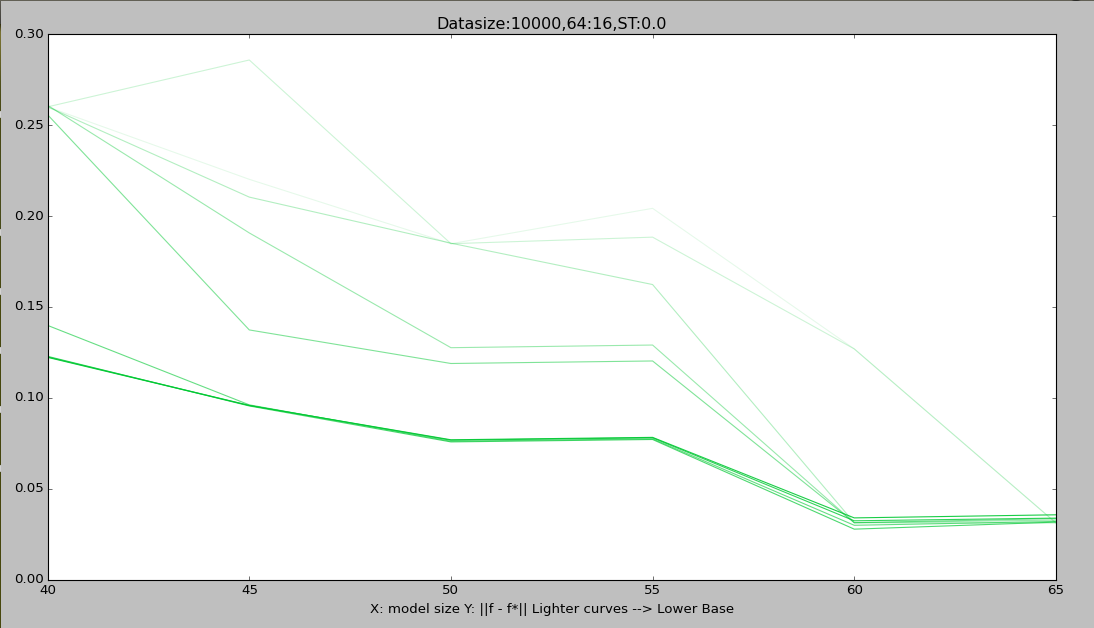
\includegraphics[width=60mm]{lucasplots/doubleloop0.png}
\caption{No noise \label{overflow}}
\end{figure}


\begin{figure}[ht!]
\centering
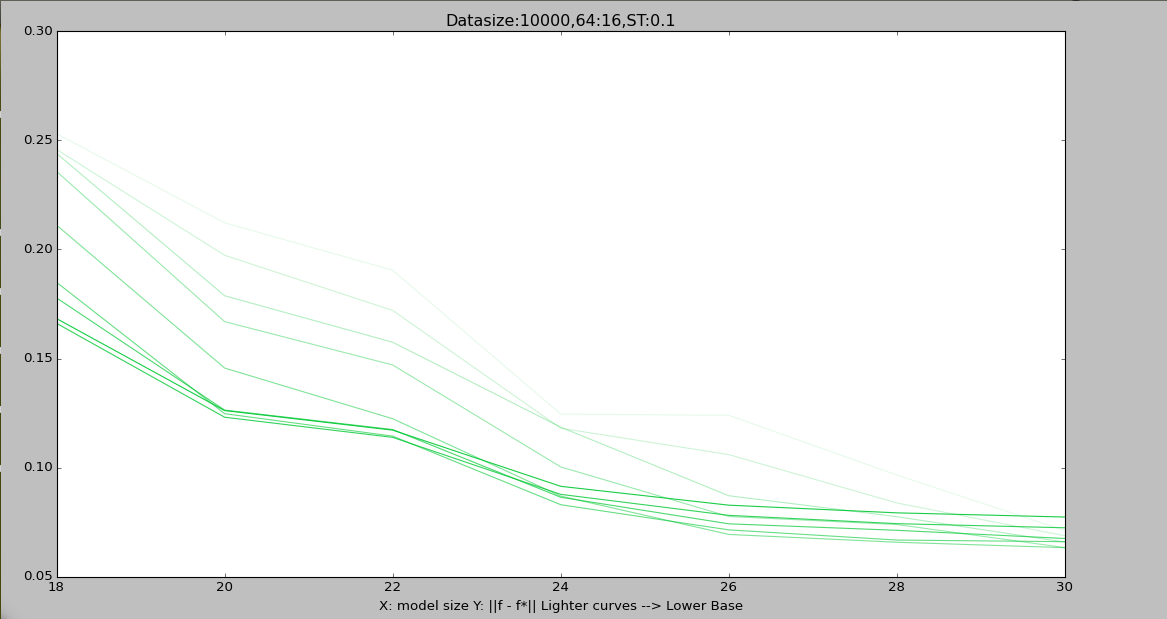
\includegraphics[width=60mm]{lucasplots/doubleloop0_1.png}
\caption{Corridor noise \label{overflow}}
\end{figure}

In both cases, the PSR with the Base System has 100 \% less error than without. In particular, we note that noise in the durations of loops doesn't harm the performance of the Base System.

\subsection{PacMan Labyrinth}

In the second experiment, we look at timing for a PacMan-Type labyrinth. In addition, we use state weightings from the learned PSRs to predict distances between the robot and objects in the environment. 

\begin{figure}[ht!]
\centering
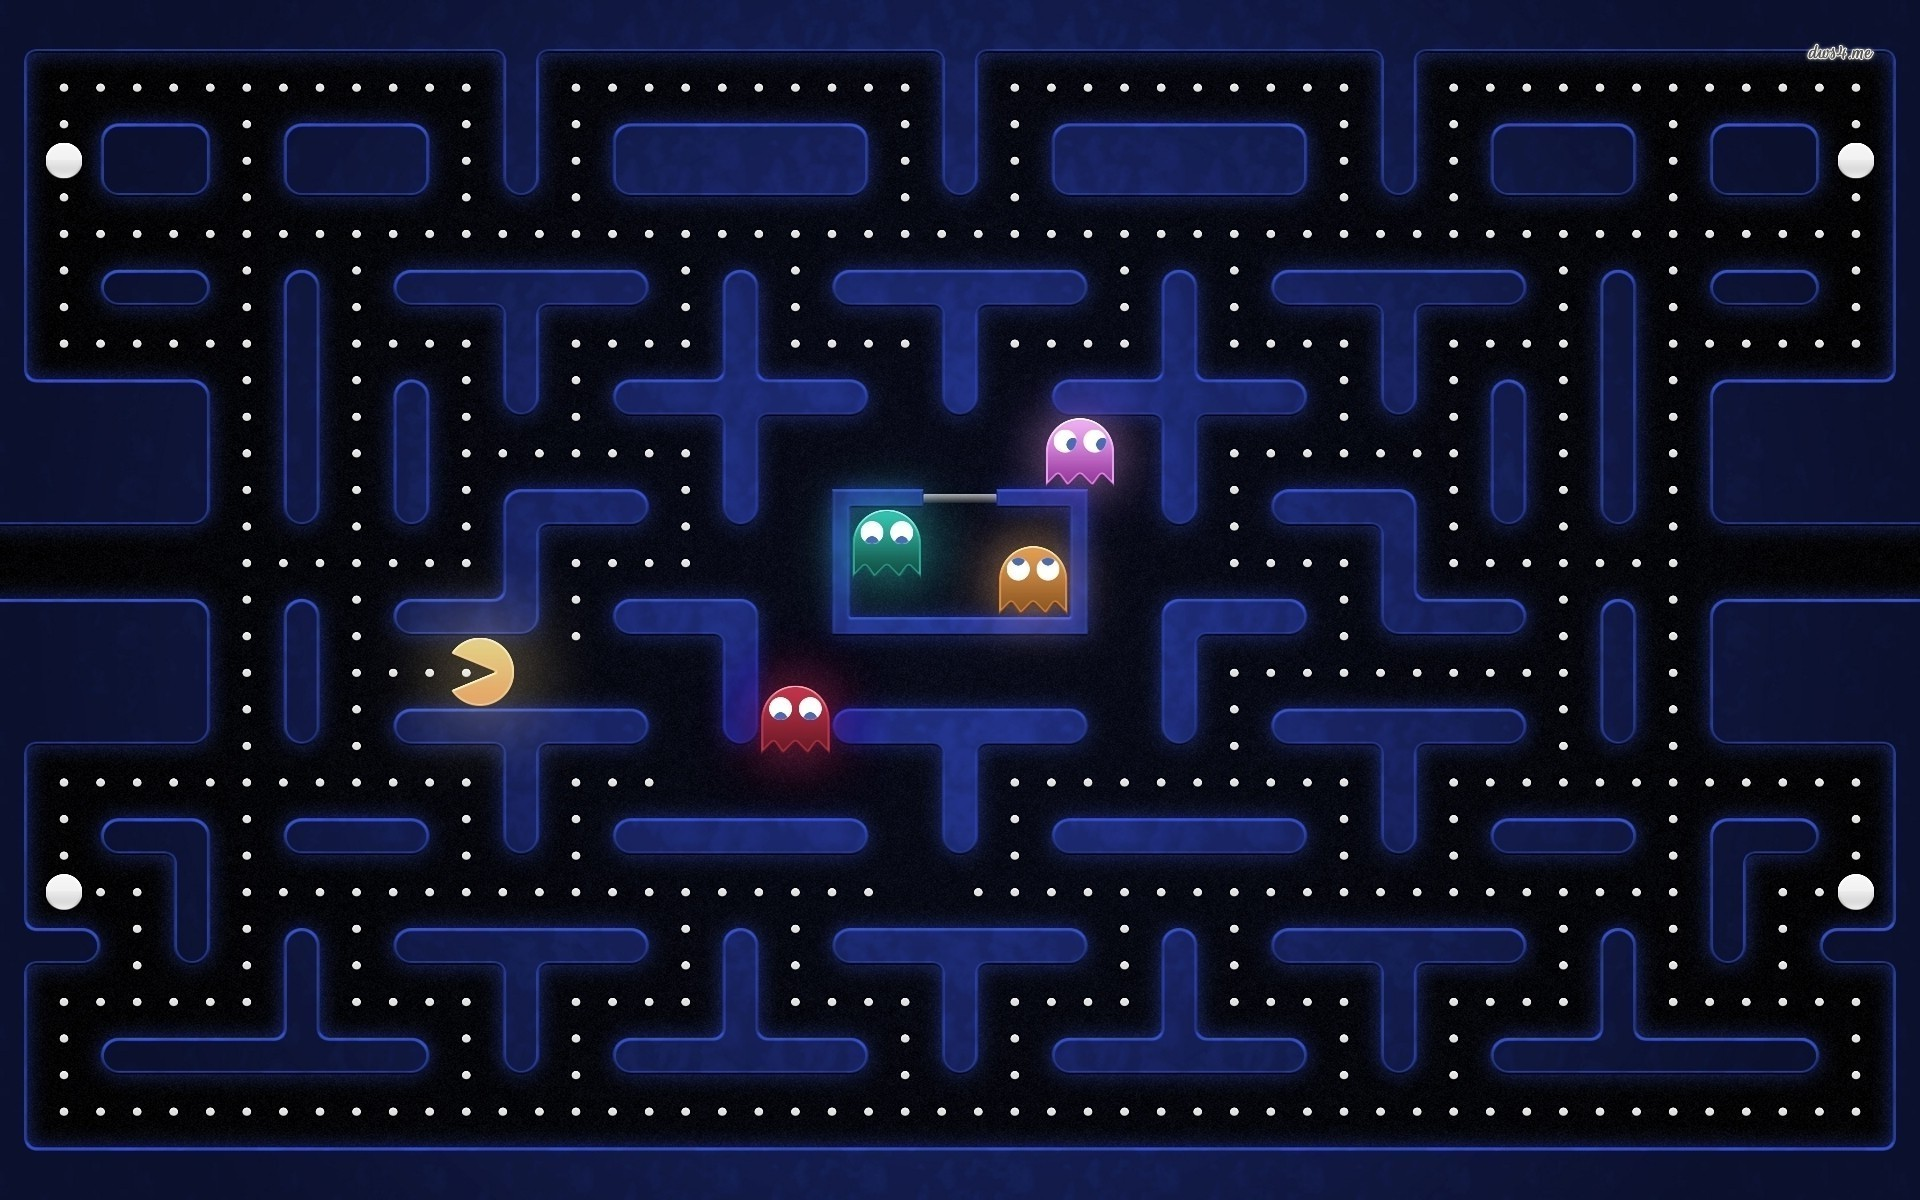
\includegraphics[width=60mm]{lucasplots/pac-man.jpg}
\caption{Pacman Environment \label{overflow}}
\end{figure}

\begin{figure}[ht!]
\centering
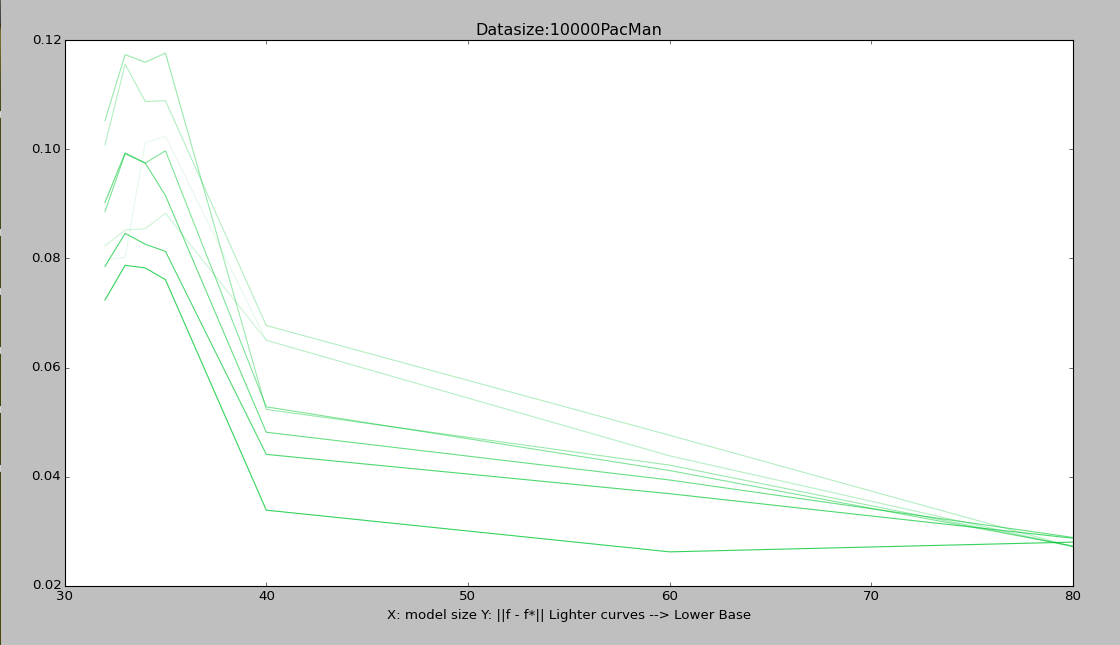
\includegraphics[width=60mm]{lucasplots/pacman10000.png}
\caption{Timing predictions in Pacman \label{overflow}}
\end{figure}


\begin{figure}[ht!]
\centering
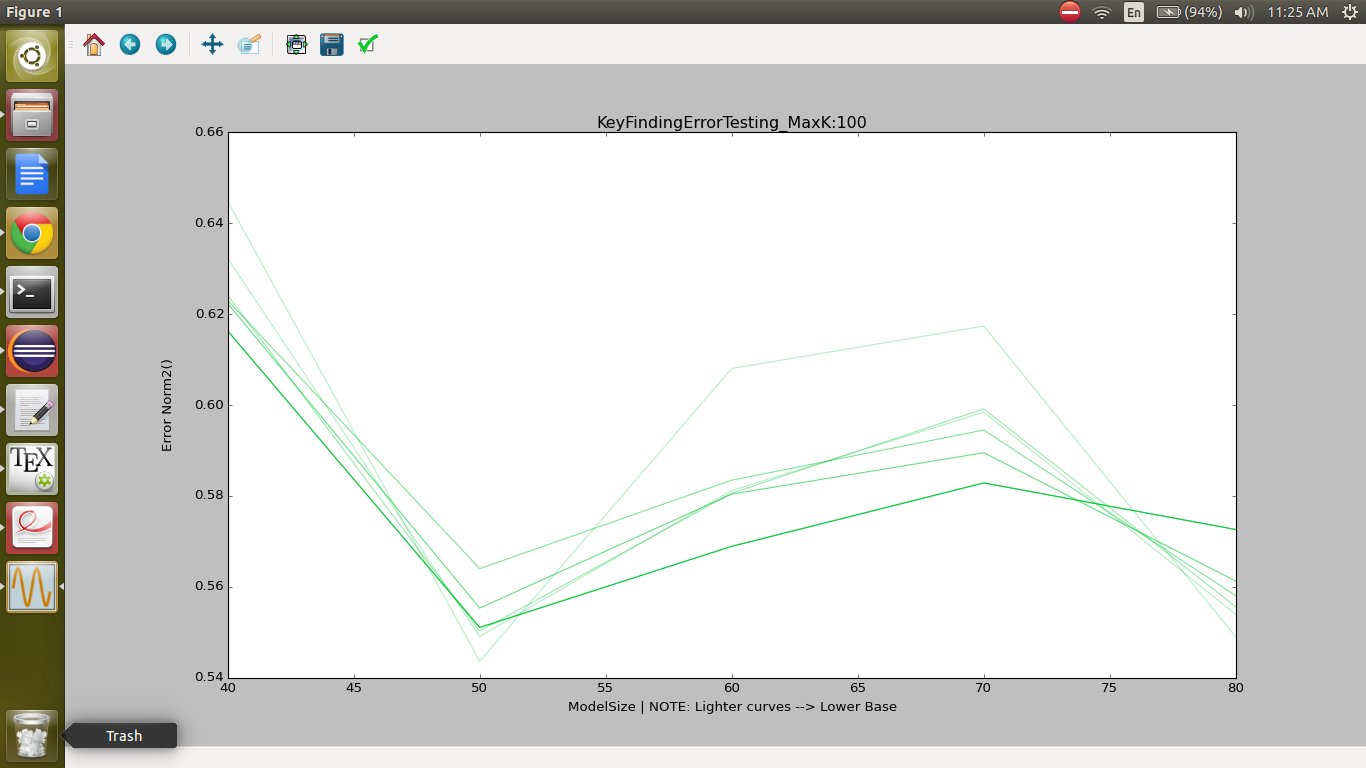
\includegraphics[width=60mm]{lucasplots/Distances.png}
\caption{Distance predictons from key \label{overflow}}
\end{figure}

Here, the Base System outperforms the naive by 100\% for timing and 45\% for distances.

\subsection{Multiple Observations}

Next, we change our set of observations to wall colors of the labyrinth. 

\begin{figure}[ht!]
\centering
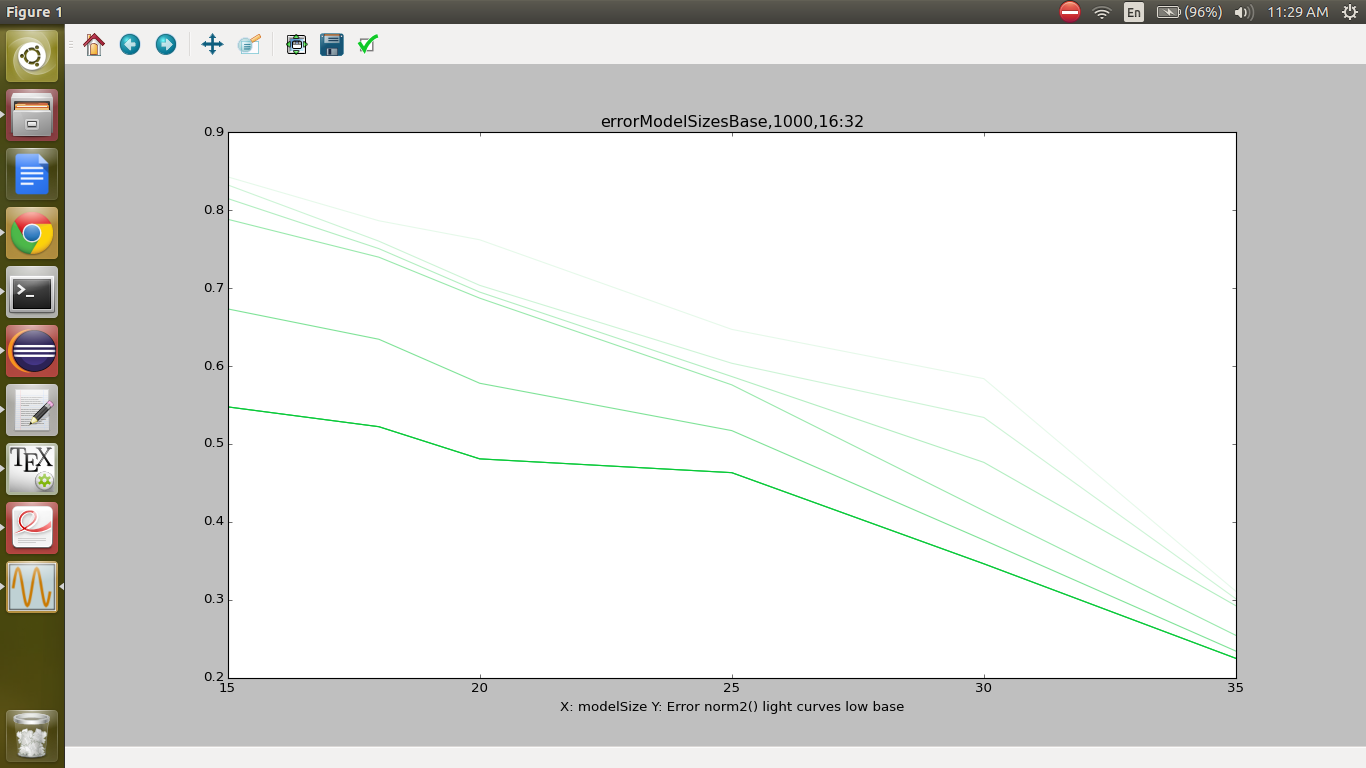
\includegraphics[width=60mm]{lucasplots/MO:16,32.png}
\caption{Predicting wall colors \label{overflow}}
\end{figure}

Here, the Base system outperforms that naive approach by 55\%. For this environment, we construct the Base System separately for each symbol. In general, one might want to use a custom heuristic to optimize the construction.

\subsection{Relevance}
The spectral framework for learning in partially observable environments has better theoretical guarantees [REFERENCE] than non-spectral methods. In this work, we showed a way to significantly improve results in practical settings, that is when one wants a smaller model. In future work, we hope to see a theoretical analysis of the apparent improvement of the Base System and optimization of it's construction.
\begin{comment}
This is \textit{italic}, \textbf{bold}, \textsc{small caps}, \textsf{sans serif}

Math is writen inside dollars: $a = b$, $a_k$, $b^s$, $a_k^j$, $a_{opt}^{\star}$ $\sin(2 \pi) = 0$, greek letters are intuitive $\alpha$, $\beta$, $\sigma$, $\Sigma$, $\Gamma$, and so on

Full line equations use 2 dollars
$$ \sum_{i=0}^{\infty} \gamma^i = \frac{1}{1-\gamma} $$

Other math symbols $a \in A \cap B \subseteq C \equiv X \sim Y \leq Z$
\end{comment}

%
% The following two commands are all you need in the
% initial runs of your .tex file to
% produce the bibliography for the citations in your paper.
\bibliographystyle{abbrv}
\bibliography{sigproc}  % sigproc.bib is the name of the Bibliography in this case
% You must have a proper ".bib" file
%  and remember to run:
% latex bibtex latex latex
% to resolve all references
%
% ACM needs 'a single self-contained file'!
%.
\subsection{References}
Generated by bibtex from your ~.bib file.  Run latex,
then bibtex, then latex twice (to resolve references)
to create the ~.bbl file.  Insert that ~.bbl file into
the .tex source file and comment out
the command \texttt{{\char'134}thebibliography}.

\end{document}



